\section{背景}

\noindent\textbf{Agent 的 ReAct 范式。}
大多数现代 Agent 工作负载都遵循 ReAct 范式 \cite{react}，即 LLM 在累积上下文上持续推理，并周期性地调用外部工具。与单轮推理不同，这种执行方式会产生长时程、多轮交互的工作流，过程中间思考、工具输出与观测结果会在几十乃至上百个步骤中不断追加到提示中 \cite{aflow,gptswarm,sppo}。

因此，如图~\ref{fig:comparisons} 所示，Agent 的上下文以及与之对应的 KV 缓存占用会在其生命周期内单调增长。这种无界且与步骤相关的增长，从根本上改变了 LLM 推理的内存与执行语义，使得 KV 缓存不再只是短生命周期的优化手段，而成为长期存在的共享系统资源。

\noindent\textbf{LLM 服务引擎中的前缀缓存。}
为了支持细粒度的前缀复用并消除冗余计算，现代 LLM 服务引擎 \cite{sglang,pagedattention} 通常将 GPU 上的 KV 缓存组织为树结构，以尽可能复用共享前缀并降低显存占用。树中的每个节点保存一段连续 token 及其对应的 KV 缓存槽。收到新请求时，系统从树根开始匹配前缀，并沿匹配路径拼接 KV 缓存槽来恢复已缓存前缀。当 GPU 显存不足时，缓存节点将通过最近最少使用（LRU）策略被淘汰。

这类设计对于由短、小且相互独立请求构成的工作负载很有效，因为此类负载的前缀复用稳定且生命周期短。然而在 Agent 批量推理中，KV 缓存需求既是长期存在的，又高度动态，而淘汰决策仍然完全依据“最近访问时间”。更详细的分析见 \S\ref{sec:motivation}。

为缓解 GPU 显存压力，许多系统还会引入 CPU 内存作为二级缓存层，将被淘汰的 KV 缓存槽通过 PCIe 卸载出去。虽然在隔离场景下，卸载通常比重计算更快 \cite{Ragcache,CachedAttention,mooncake,sppo,internevo}，但在高并发下，这种优势会显著下降。并发的卸载与重新加载会争抢 PCIe 带宽，并引入额外同步开销，导致每一步的时延像图~\ref{fig:comparisons}c 那样迅速上升。这表明，为低并发或请求中心型工作负载设计的 KV 缓存管理策略，在 Agent 批量推理中很可能表现不佳。

\begin{figure}[tb]
    \centering
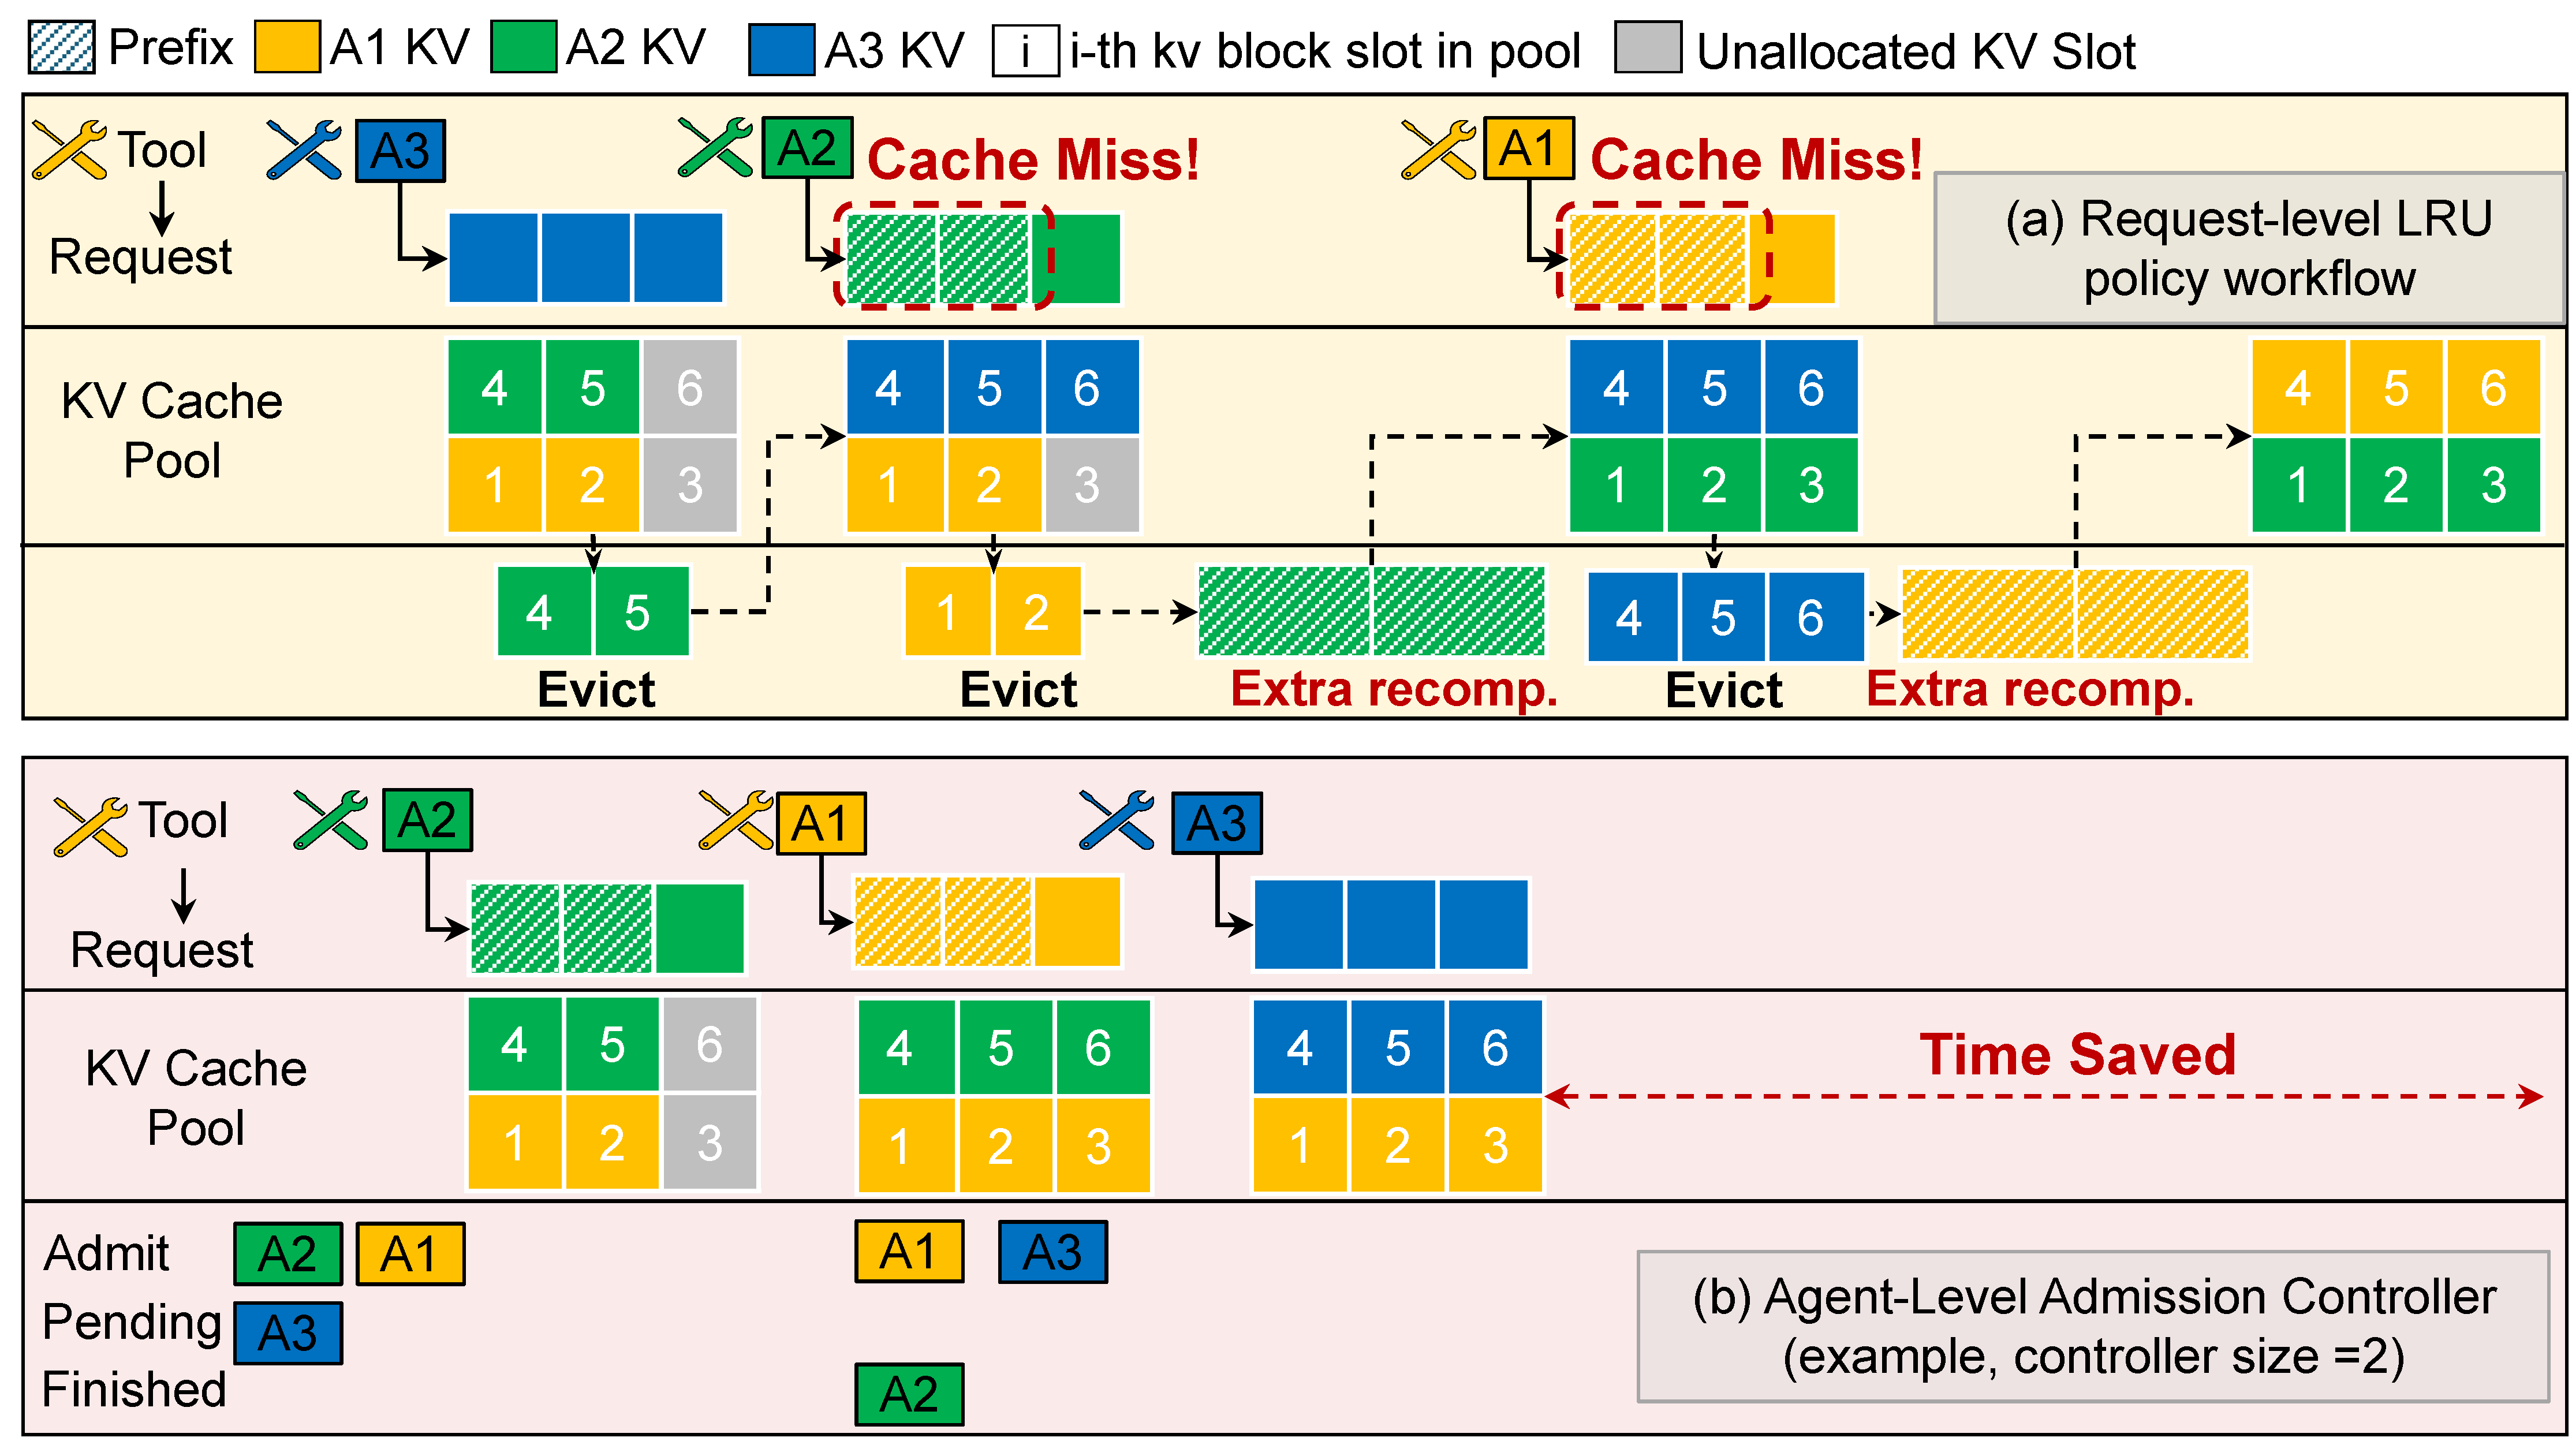
\includegraphics[width=0.98\linewidth]{figure/3agents.pdf}
    \caption{三 Agent 工作流示意图，展示中期抖动与 Agent 级准入控制。(a) LRU 淘汰使暂停中的 Agent 丢失 KV 缓存，从而触发反复重计算并导致中期抖动。(b) Agent 级准入控制通过限制并发度避免缓存过量承诺与淘汰引发的重计算。}
    \label{fig:twoagent}
\end{figure}

\noindent\textbf{拥塞控制与 AIMD。}
拥塞控制长期以来一直被视为分布式系统中调节对共享、有限资源访问的经典机制 \cite{congestion_control}。在分组交换网络中，多个发送方会争用有限链路带宽，如果发送行为缺乏协调，就会引发拥塞崩溃。为此，TCP 拥塞控制会根据能够表征拥塞的反馈信号（如丢包或往返时延增加）动态调整发送速率。

最常见的方法之一是加性增大、乘性减小（AIMD）算法 \cite{chiu1989analysis,AIMD1}。当系统未观察到拥塞时，发送方以较小的加性步长增加拥塞窗口 \cwnd\footnote{\cwnd 是发送端的一个上限，用来控制一次可以发送多少数据，以避免压垮网络。}，以谨慎探测额外可用容量；一旦检测到拥塞，则通过乘性方式缩减 \cwnd，从而快速释放共享资源上的压力。由于其简单且有效，AIMD 已广泛用于网络系统、数据中心调度与分布式存储等场景 \cite{tcp}。

本文将这种思想类比到 Agent 批量推理中的 GPU 驻留 KV 缓存容量。类似于网络链路，KV 缓存也是共享且有限的资源，一旦过量承诺，就会以效率下降、内存碎片化和执行时延上升的形式表现为“拥塞”。不同之处在于，LLM 推理中的拥塞信号更间接，也更滞后，因为资源使用是以 Agent 执行粒度演化的，而不是按 token 独立变化。正因如此，我们需要在 Agent 级别重新解释拥塞控制原则，并据此调节准入，从而在 Agent 批量推理中维持高吞吐。
